% !TEX encoding = UTF-8 Unicode
\documentclass[12pt,oneside]{fithesis2}
\usepackage[english]{babel}       % Multilingual support
\usepackage[utf8]{inputenc}       % UTF-8 encoding
\usepackage[T1]{fontenc}          % T1 font encoding
\usepackage[                      % A sans serif font that blends well with Palatino
  scaled=0.86
]{berasans}
\usepackage[                      % A tt font if you do not like LM's tt
  scaled=1.03
]{inconsolata}
\usepackage[                      % Clickable links
  plainpages = false,               % We have multiple page numberings
  pdfpagelabels                     % Generate pdf page labels
]{hyperref}
\usepackage{blindtext}            % Lorem ipsum generator
\usepackage{graphicx}
\usepackage{svg}
\usepackage{amsmath}
\usepackage{hyperref}
\usepackage{tikz}
\usepackage{pgfplots}
\usepackage{pgfplotstable}
\usepackage{float}

\thesislang{en}                   % The language of the thesis
\thesistitle{Time Series Prediction Using Neural Networks}       % The title of the thesis
\thesissubtitle{Bachelor Thesis}  % The type of the thesis
\thesisstudent{Karol Kuna}          % Your name
\thesiswoman{false}                % Your gender
\thesisfaculty{fi}                % Your faculty
\thesisyear{Spring \the\year}     % The academic term of your thesis defense
\thesisadvisor{doc. RNDr. Tomáš Brázdil, Ph.D.}   % Your advisor

%\DeclareMathSizes{14}{14}{8}{8} %display/text style, script style and scriptscript style.

\begin{document}
  \FrontMatter                    % The front matter
    \ThesisTitlePage                % The title page
    \begin{ThesisDeclaration}       % The declaration
      \DeclarationText
      \AdvisorName
    \end{ThesisDeclaration}
    \begin{ThesisThanks}            % The acknowledgements (optional)
      I would like to thank my advisor for the guidance he has provided. %TODO
    \end{ThesisThanks}
    \begin{ThesisAbstract}          % The abstract
      This thesis compares existing methods for predicting time series in real time using neural networks. Focus is put on recurrent neural networks (RNNs) and online learning algorithms, such as Real-Time Recurrent Learning and truncated Backpropagation Through Time. In addition to the standard Elman's RNN architecture, \mbox{Clockwork-RNN} is examined. Methods are compared in terms of prediction accuracy and computational time, which is critical in real-time applications. Part of the work is experimental implementation of the tested models and working applications in robotics and  network traffic monitoring.
    \end{ThesisAbstract}
    \begin{ThesisKeyWords}          % The keywords
	time series, prediction, neural network, recurrent network, backpropagation, backpropagation through time, real-time recurrent learning, clockwork recurrent network
    \end{ThesisKeyWords}
    \tableofcontents                % The table of contents
   \listoftables                   % The list of tables (optional)
   \listoffigures                  % The list of figures (optional)
   
  
  \MainMatter
    \chapter{Introduction} %what is prediction and anomaly detection, why   
Each year more and more data is collected from high velocity data streams. Machine learning algorithms are used to analyse and create models of the data. Patterns found in the data structure are then exploited to make predictions about the future which can be used to guide decision making. In this thesis, I compare various artifical neural network (ANN) architectures and learning algorithms for online prediction of time series.

\par %neural networks, modelling data?
One of the most popular machine learning algorithms are ANNs which are capable of approximating unknown functions and thus are good candidates for use in prediction. Inspired by biological neural networks, ANNs consist of artificial neurons wired together to form a network.
\par %which networks are compared
Common architectures, such as feedforward networks (FFN) and simple recurrent networks (SRN) trained by backpropagation through time (BPTT) and Real-Time Recurrent Learning (RTRL), as well as latest Clockwork-RNN are evaluated in this thesis. Algorithms are compared in terms of prediction accuracy as well as computational time and the trade-off between them.
\par %what are time series
Time series are sequences of data points in time, usually created by measuring output of some process in discrete time intervals. The goal of prediction is to successfully estimate output of the process in next time step or several steps. It is assumed that the process is at least partially observable and to some extent, future values can be determined by observing past values. Prediction then reduces to problem of process approximation.
\par %describe the value of online prediction
Since value of stored data decreases over time, effort is put into gaining insight from data as they come. Many applications don't require storing data at all, or storing it would be impractical, therefore it is advantageous to create models and update them with every data point. Continuous online learning is well suited for such tasks and can adapt to changing environments without human intervention.
\par %applications described in this thesis, TODO: add citations. scenarios or applications?
Quality and speed of prediction is tested in two application scenarios. The first is robotic simulator implemented in 3D physics library BEPUPhysics. Manipulator with three actuated joints is created, the goal is to predict future position of robot's arm. The prediction network should act as a virtual model of the body, which can be useful in control systems, e.g. internal model control.

%Data points that do not conform to the learned model of normal behaviour are called anomalies. Detecting anomalies is found to be increasingly important in computer network security. An anomaly may signal unexpected events, such as computer being under denial of service attack or unforeseen load.

\par %anomaly detection in network
The second scenario is monitoring utilisation of computer resources, namely processor, memory, disk, and network usage. Network should constantly predict future values of these variables and detect anomalies. Should an unexpected event occur, it needs to be logged for an administrator to examine.
\par

\chapter{Prediction}
\section{Time Series}
Time series are sequences of data points measured over time. In this thesis, data points are real-valued vectors implemented as arrays of floating point numbers. Data sequence is created by measuring output of a process at discrete, regular time intervals. %discrete?
Process may also receive input in every time step, which affects its future behaviour, or it may be purely generative receiving no input at all. For generalisation's sake, let's assume every process receives input which is a real-valued vector just like output. Generative processes then simply receive input vector of zero length.
	\begin{figure}[ht]
		\centering
		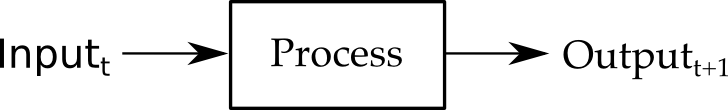
\includegraphics[width=182px]{process.png}
		\caption{Schema of a process.}
	\end{figure}
In every time step, process receives input, updates its internal state and produces output. Internal state of the process is usually hidden and can be observed only partially from output of the process. %any assumptions?

\section{Prediction}
The goal of prediction is to approximate the process as closely as possible and hence minimise forecast error, i.e. difference between actual and forecasted value. Naive approaches include methods like averaging past data points, returning previous data point or linear extrapolation. While these methods may suffice for some very simple time series, more sophisticated methods are required to cope with real-world time series. Sophisticated methods use historical data to estimate future value by finding a model of the process that empirically fits past data. \par
The problem of prediction can be alternatively viewed as problem of function approximation.
	$$\left(State_{t+1}, Output_{t+1}\right) = Process(State_t, Input_t)$$
Process is a function from current internal state and input to next internal state and output. Unfortunately, internal state is unknown, so next output can only be estimated from history of inputs and outputs. History can be defined as an ordered set of past inputs and outputs.
	$$History_t = \left( (Input_{t}, Output_{t}), (Input_{t-1}, Output_{t-1}), \dots (Input_{0}, Output_{0}) \right)$$
Prediction is then a function from current history to next output.
	$$Output_{t+1} \approx Prediction( History_t )$$

\section{Prediction Horizon}
Number of steps the prediction is made into the future is called prediction horizon. Some applications require estimating output of the process more than one step into the future. This can be achieved by chaining one step predictions or by approximating function:
	$$Output_{t+h} \approx Prediction( History_t, FutureInputs )$$

\section{Prediction Chain}
%rephrase this
As an alternative for predicting multiple steps of the future, one step prediction can be applied recursively multiple times, i.e. predict next step, from the prediction predict next step etc. Intermediary results are then available for use. In case of processes that receive input, chaining predictions is suitable only if the future inputs are known up until prediction horizon.
%TODO: fix this formula
$$Output_{t+h} \approx Prediction( Prediction(  \dots Prediction(State_t, Input_t), Input_{t+1} ) \dots Input_{t+h} )$$


\chapter{Artificial Neural Networks}
Inspired by biological neural networks, ANNs are groups of elementary processing units called artificial neurons connected together to form a directed graph. Nodes of the graph represent biological neurons and connections between them represent synapses. Unlike in biological neural networks, connections between artificial neurons cannot be added or removed after the network was created. Instead, connections are weighted and the weights are adapted by learning algorithm. \par

Input signal propagates through the network in the direction of connections until it reaches output of the network. In supervised learning, learning algorithm adapts the weights in order to minimize the difference between output of the network and desired output provided by teacher.

\section{Artificial Neuron}
The complex behavior of biological neurons was simplified to create a mathematical model of artificial neurons, also called units. Each unit consists of a real valued activation representing some property of the unit. Unit receives activations of other units via input connections, computes its output activation and sends it to other units. \par
Connections between units are stored in a matrix $w$, where $w_{ij}$ denotes weight of the connection from unit $i$ to unit $j$. Every unit $j$ has a potential $p_j$ which is calculated as weighted sum of all of its $N$ input units and bias. \par

$$p_{j} = \sum\limits_{i = 1}^{N+1} w_{ij} a_{i}$$

Bias term, also known as threshold unit, is usually represented as an extra input unit whose activation always equals one. Presence of bias term enables shifting the activation function along x-axis by changing the weight of connection from threshold unit.

Activation of the unit $a_j$ is then computed from the potential $p_j$ transformed by a non-linear activation function $act$.

$$a_{j} = act\left(p_j\right)$$
\par
Commonly used non-linear activation function ranging from 0 to 1 is sigmoid function thanks to its easily computable derivative which is used by learning algorithms.

$$\sigma(x) = {1 \over {1 + e^{-x}}}$$
$${{d\sigma(x)} \over dx} = \sigma(x)  \left(1 - \sigma(x)\right)$$

\section{Feedforward Neural Networks}
Feedforward neural network is an ANNs where information moves in one direction, from input to output, i.e. without any backward or recurrent connections. Multilayer perceptron (MLP) is a class of feedforward networks consisting of three or more layers of units. Layer is a group of units receiving connections from the same units. Units inside a layer are not connected to each other. \par
	\begin{figure}[ht]
		\centering
		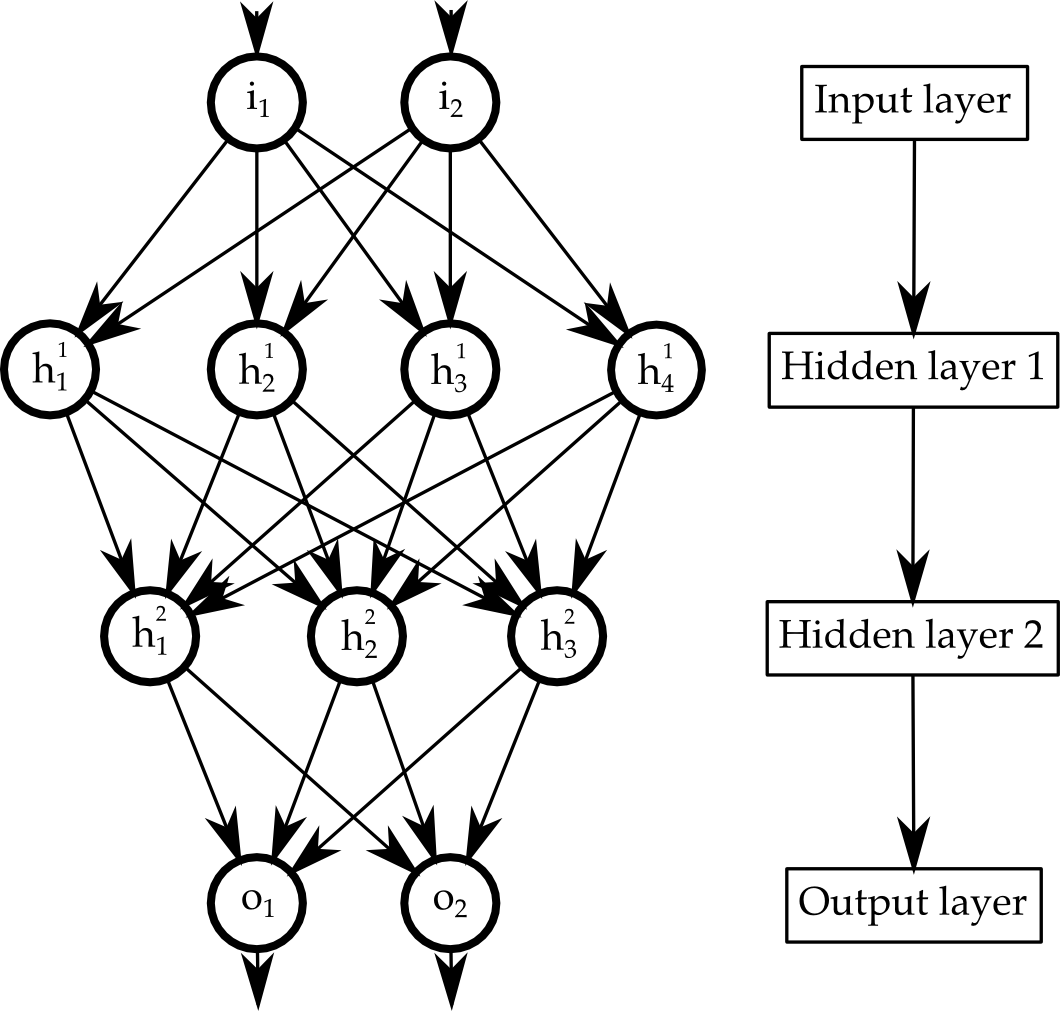
\includegraphics[width=265px]{mlp.png}
		\caption{On the left, MLP consisting of input layer with two units, two hidden layers with four and three units respectively, and output layer with two untis. Schematic diagram of the MLP's layers on the right.}
	\end{figure}
MLP consists of three types of layers: input layer, one or more hidden layers and output layer. Input layer is the first layer of network and it receives no connections from other units, but instead holds network's input vector as activation of its units. Input layer is fully connected to first hidden layer. Hidden layer $i$ is then fully connected to hidden layer $i + 1$. Last hidden layer is fully connected to output layer. Activation of output units is considered to be output of the network. \par
MLPs are often used to approximate unknown functions from their inputs to outputs. MLP's capability of approximating any continuous function with support in the unit hypercube with only single hidden layer and sigmoid activation function was first proved by George Cybenko \cite{universal-approx-theorem}.

\subsection{Backpropagation}
Backpropagation, or backward propagation of errors, is the most used supervised learning algorithm for adapting weights of feedforward ANNs. Weights of the network are tuned so as to minimize summed squared error
$$E = {1 \over 2}(t - o)^2$$
where $t$ denotes target output provided by teacher and $o$ is network's prediction of the output for the corresponding input. \par
Let's assume the error is a function of network's weights, then backpropagation can be seen as optimization problem and standard gradient descent method can be applied. Local minimum is approached by changing weights along the direction of negative error gradient 
$$-{{\partial E} \over {\partial w}}$$
proportionally to $\alpha$, which is constant positive value called learning rate.
$$new \; w_{ij} = w_{ij} - \alpha {{\partial E} \over {\partial w_{ij}}}$$

The central part of the algorithm is finding the error gradient. Let's assume there is a MLP with $L$ layers, first being input and last being output layer. Layer $k$ has $U_k$ units and holds a matrix of weights $w_{ij}^k$ representing weights of connections from unit $i$ in layer $k - 1$ to unit $j$ in layer $k$. The computation can be then divided into three steps:

\begin{enumerate}
  \item Forward propagation. Input vector is copied to activation of input layer. Layer by layer, from first hidden to output layer, activation of units is calculated. Activation of the output layer $a^L$ is considered output of the network.
  
  \item Backward propagation. Compute error gradient $\Delta^L_i$ w.r.t. unit $i$ for each output layer unit $i$ as
  $$\Delta^L_i = \left(target_i - a^L_i\right){{\partial{act\left(p^L_i\right)}} \over {\partial p^L_i}}$$
  For units $i$ of hidden layers $h = L-1,\; L-2,\;  \dots 2$, error term is
  $$\Delta^h_i = \sum\limits_{j=1}^{U_{h + 1}} \Delta_{j}^{h+1}w_{ji}^{h} {{\partial{act\left(p^h_i\right)}} \over {\partial p^h_i}}$$
  
  \item Weights update. Change weights in layer $k$ according to
  $$new \; w_{ij}^k = w_{ij}^k + \alpha \Delta_i^{k+1} a_{j}^{k}$$

\end{enumerate}

%conclusion about backprop

\subsection{Time-Delay Neural Networks}
Time-Delay Neural Network (TDNN) is a modification of feedforward network designed to capture dynamics of modelled process \cite{phoneme-recognition-tdnn}. As FFNs have no internal memory to store information about past, they are insufficient for processing temporal sequences. To overcome this, memory of past is introduced by means of extending network's input with sliding window of previous inputs, also known as tapped delay line. The information about the past is thus stored in the network input itself. Because there are no modifications to the network, standard backpropagation algorithm can be used.\par
Size of the sliding window determines how many past inputs are stored and consequently how much past data can be correlated to future output. Too small window may not capture necessary dynamics of the system, because network is blind to anything that happened before, and thus create inferior results. Whereas too large window can drastically prolong learning time.\par
To generalise TDNN to processes that also receive input, prediction of future process output can be defined as approximation of function $Predict$ with window size $w$
$$Output_{t+1} = Predict(Output_t, \dots, Output_{t-w}, Input_t, \dots Input_{t-w})$$

\section{Recurrent Neural Networks}
Recurrent network is a class of ANNs which allows units to form a directed graph with cycles. This allows the network to store an internal state and consequently process sequences of inputs and thus perform temporal tasks.



\subsection{Elman's Simple Recurrent Network}
One of the simplest and most popular RNN architectures is Elman's  simple recurrent network (SRN). SRN resembles a three-layer feedforward network due to its structure composed of input, hidden and output layer, with addition of a context layer. Input and context layer project to hidden layer, which projects to output layer. Context layer is a copy of hidden layer's activation in previous time step. Therefore, context layer acts as network's memory of previous activity.

	\begin{figure}[ht]
		\centering
		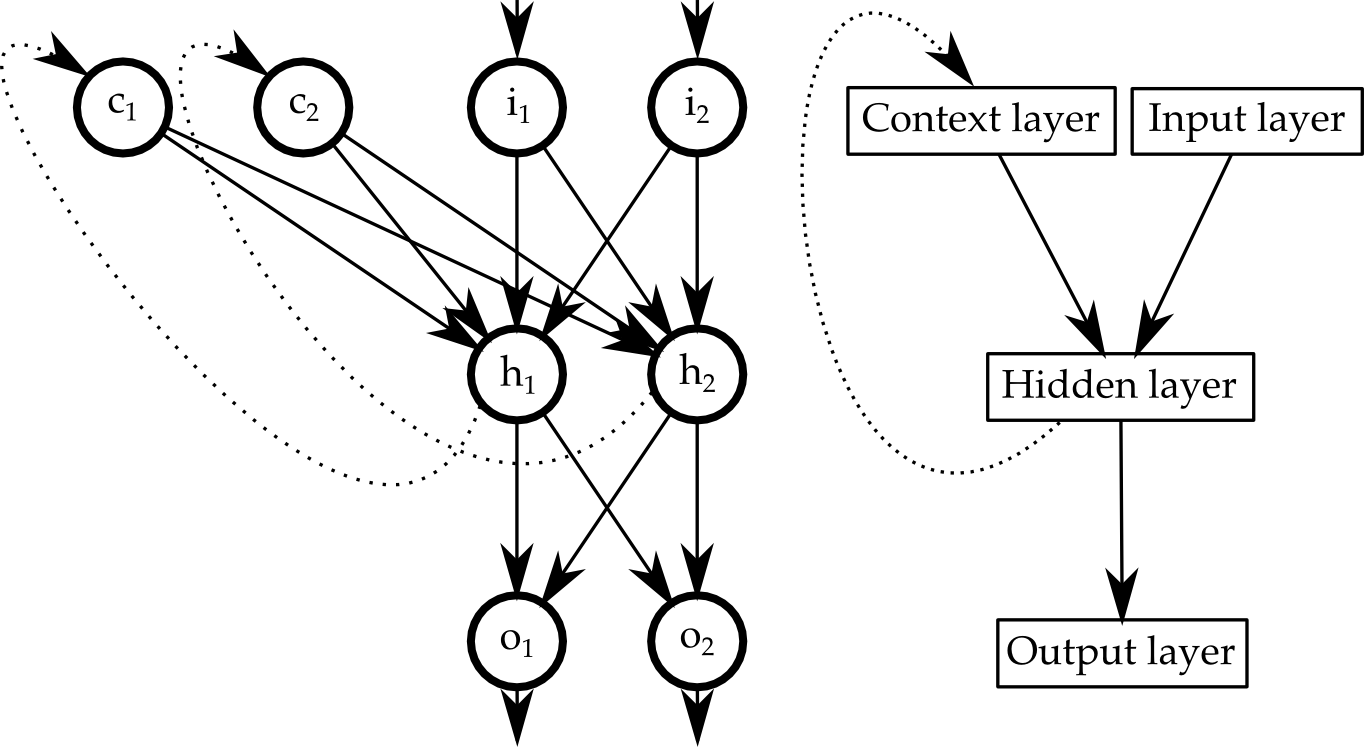
\includegraphics[width=341px]{elman-rnn.png}
		\caption{On the left, Elman's recurrent network with input, hidden, context, and output layer, each containing two units. On the right, schema of layers in Elman network. Dotted link signifies copying activity of source's units to target units.}
	\end{figure}

Recurrent network's dynamics can be formulated by two equations:
$$a^{hid}(t) = act\left( W^{in}a^{in}(t) + W^{hid} a^{hid}(t-1)\right)$$
$$a^{out}(t) = act\left( W^{out}a^{hid}(t)\right)$$
where $a^{in}(t)$, $a^{hid}(t)$ and $a^{out}(t)$ are column vectors of activations of units in input, hidden and output layer respectively in time step $t$. $W^{in}$, $W^{hid}$ and $W^{out}$ are matrices \footnote{Element at row $i$ and column $j$ of the matrix W holds weight of connection from unit $j$ to unit $i$} of weights of connections from input to hidden layer, hidden to hidden layer and hidden to output layer respectively. $act$ is an element wise activation function.\par

	
\subsection{Backpropagation Through Time}
Standard backpropagation algorithm is not suited for networks with cycles in them. Fortunately, RNN can be modified to look like a feedforward network by unfolding the network in time as shown in figure 3.3 and then trained with Backpropagation Through Time (BPTT) algorithm first laid out by Rumelhart, Hinton and Williams in 1986 \cite{rumelhart-hinton-williams}.\par

The unfolding process begins with a SRN in current time step $t$, denoted as $SRN_t$. Since context layer of a SRN is just a copy of hidden layer activation from previous step, cycles in the network can be avoided by replacing context layer with an identical copy of the SRN network from previous step, $SRN_{t-1}$. Hidden layer of $SRN_{t-1}$ is then connected to hidden layer of $SRN_t$. This procedure is repeated until time step $0$ is reached, in which case the context layer is not replaced, but rather stays set to its initial activity. The number of SRN copies represents depth of the unfolded network and each copy of the network uses exact same set of weights.\par

	\begin{figure}[ht]
		\centering
		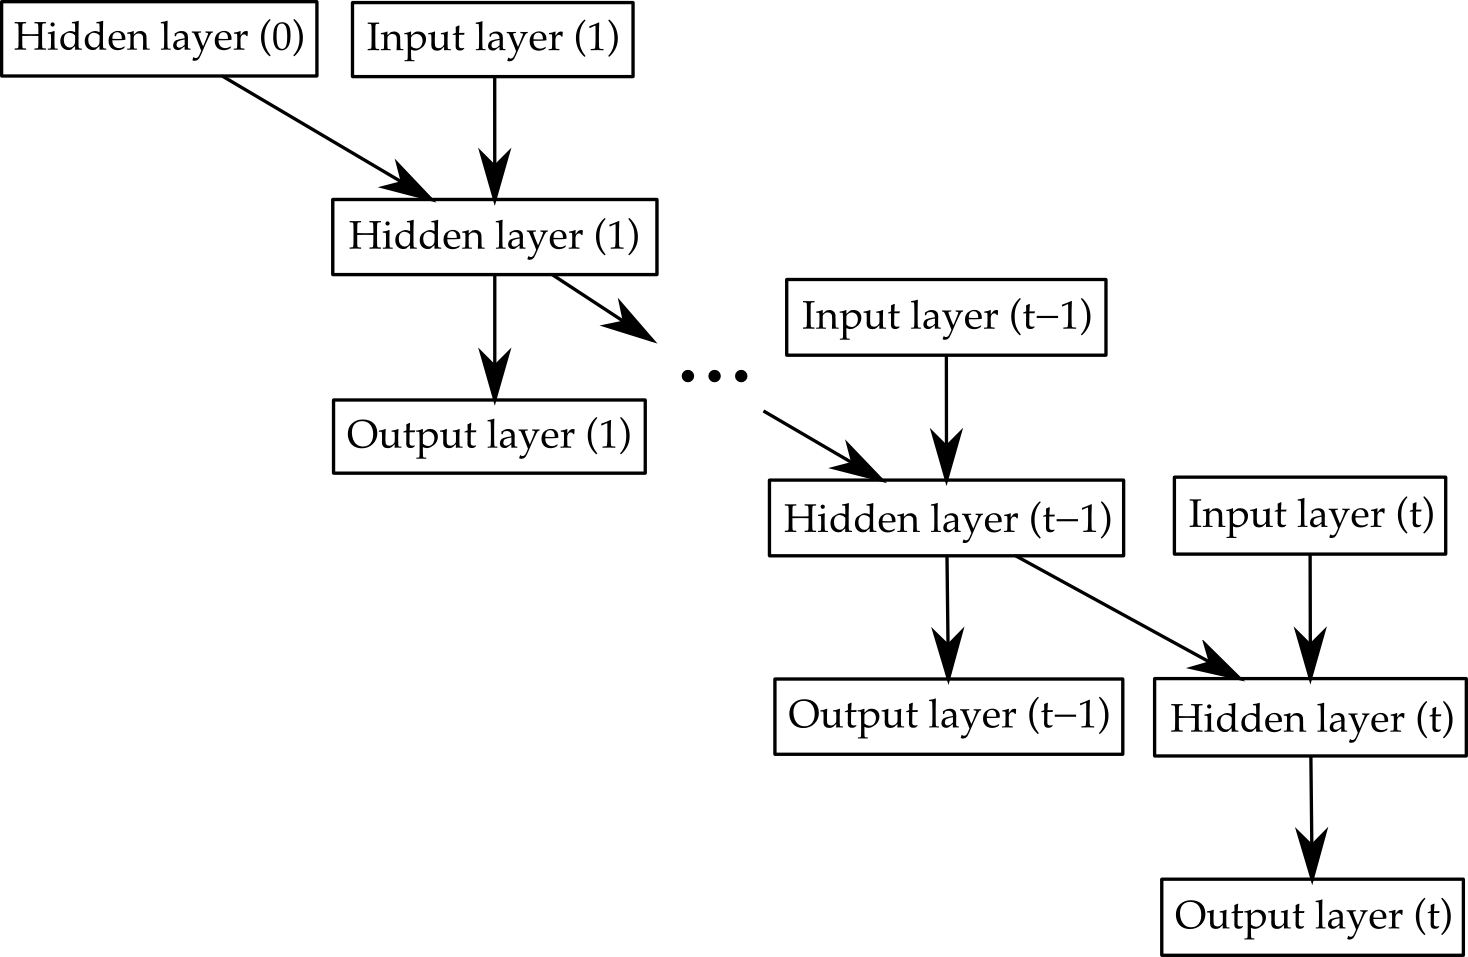
\includegraphics[width=367px]{bptt2.png}
		\caption{Elman's recurrent network unfolded in time. }
		\label{fig:bptt}
	\end{figure}

Once the SRN has been unfolded into a feedforward network, backpropagation can be used. The algorithm again consists of 3 steps:
\begin{enumerate}
  \item Forward propagation. Signal is propagated through the unfolded network in the standard fashion, from top to bottom. In this case, from the SRN copy furthest in the past to the most recent copy.
  \item Backward propagation. Error gradient $\Delta^{out}_{i}(t)$ of every output layer of SRN copy in time $t$ is computed w.r.t. output unit $i$ as:
 
  $$\Delta^{out}_{i}(t) = \left(target_{i}(t) - a^{out}_{i}(t)\right) {{\partial{act\left(a^{out}_{i}(t)\right)}} \over {\partial a^{out}_{i}(t)}}$$
 
 
  For every unit $i$ in hidden layer of unfolded SRN in time step $t$, let $\Delta_1 \dots \Delta_N$ be error terms of units that receive connections from hidden layer in time $t$. Error term $\Delta^{hid}_{i}(t)$ w.r.t. hidden unit $i$ is then
  %check wij or wji
  $$\Delta^{hid}_{i}(t) =\left(\sum\limits_{j=1}^{N} \Delta_{j}w_{ij}^{h}\right) {{\partial{act\left(a^{hid}_{i}(t)\right)}} \over {\partial a^{hid}_{i}(t)}}$$
  
  \item Update weights in the original SRN. For every unit $i$ of the original network $k$ that is connected to units $j$ in layer $l$, update the weight according to
  %finish this
  $$new \; w_{ij}^l = w_{ij}^l + \alpha \sum\limits_{m=1}^{t} \Delta_i^{k}\left(m\right) a_{j}^{l}\left(m\right)$$

\end{enumerate}

%close this section by something general about BPTT

\subsection{Truncated Backpropagation Through Time}

Number of SRN copies in the unfolded network is equal to current time step $t$. Should this algorithm be used in online manner, it would be impractical, since its memory footprint would grow linearly with time. To overcome this, online version of the BPTT algorithm called Truncated Backpropagation Through Time (TBTT) can be used. TBPTT works analogously to BPTT, except the maximum depth of the unfolded network is limited.\par
%TODO: be more specific, what about running every nth step

\subsection{Real-Time Recurrent Learning}
Real-Time Recurrent Learning (RTRL) algorithm is a gradient descent method suitable for online learning of recurrent networks.\par

%rephrase or replace "denoted" by synonym
Let's assume the recurrent network's total number of $U$ units is divided into $U_{in}$ input units, $U_{hid}$ hidden units and $U_{out}$ output units. For convenience, let's denote potential and activation of all units by $p_i$ and $a_i$, where $i=1 \dots U_{in}$ represents indices of input units, $i=U_{in} + 1 \dots U_{in} + U_{hid}$ represents indices of hidden units and $i=U_{in} + U_{hid} + 1 \dots U_{in} + U_{hid} + U_{out}$ represents indices of output units. All weights of connections from unit $i$ to unit $j$ can be then denoted by $w_{ij}$.\par

We wish to minimise error $E$ in time step $t$ %what about global error?
$$E(t) = {1 \over 2}\left(a_i(t) - target_i(t)\right)^2$$
where $i$ enumerates indices of output units and $target$ holds teacher given desired activations of output units. We do this by adjusting weights along the negative gradient of error
$$-{{\partial E(t)} \over {\partial w_{ij}}} = \sum\limits_{k=U_{in}+U_{hid}+1}^U \left( target_i(t) - a_i(t) \right) {{\partial a_i(t)} \over {\partial w_{ij}}}$$
${\partial a_i(t)} / {\partial w_{ij}}$ can be computed by differentiating the network dynamics equation, resulting in the derivative $v^k_{ij}$ of hidden or output unit $k$ w.r.t. weight $w_{ij}$
$$ v^k_{ij}(t+1) = {{\partial a_k(t+1)} \over {\partial w_{ij}}} = act'(p_k(t)) \left[ \left(\sum\limits_{j=U_{in+1}}^{U}  w_{kj} {{\partial a_j(t)} \over {\partial w_{ij}}}\right) + \delta_{ki} act_j(t) \right] $$
where $\delta_{ki}$ is Kronecker's delta
$$\delta_{ki} =
    \begin{cases}
            1, &         \text{if } k=i,\\
            0, &         \text{if } k\neq i.
    \end{cases}$$
This creates dynamical system with variables $v^k_{ij}$ for all hidden and output units \cite{williams-zipser}. Since the initial state of the network is independent from its weights, we can set $v^k_{ij}(0) = 0$. Network's weights are then updated according to negative gradient of the error
$$new \; w_{ij} =  w_{ij} - \alpha \sum\limits_{k=U_{in}+U_{hid}+1}^U \left[ \left(a_k(t) - target_k(t) \right) v_{ij}^k \right]$$

\section{Clockwork Recurrent Network}
%add citations
SRNs have trouble capturing capturing long-term dependencies in input sequences due to vanishing gradient \cite{vanishing-gradient}. Clockwork recurrent neural network (CW-RNN) is a modification of Elman's SRN designed to solve this problem by having hidden layer split into $M$ modules running at different clocks \cite{cw-rnn}.
Each module $i$ is assigned a clock rate $T_i$. In time step $t$ only modules with period $T_i$ that satisfies $(t \; mod \; T_i) = 0$ compute its activation, other modules retain their previous activation.  \par

Like in SRN, input layer is connected to hidden layer, context layer stores activation of hidden layer from previous time step and hidden layer is connected to output layer. The difference is that module of hidden layer with clock rate $T_i$ connects to module in context layer with period $T_j$ only if $T_i <= T_j$ as shown in figure 3.4.
	\begin{figure}[ht]
		\centering
		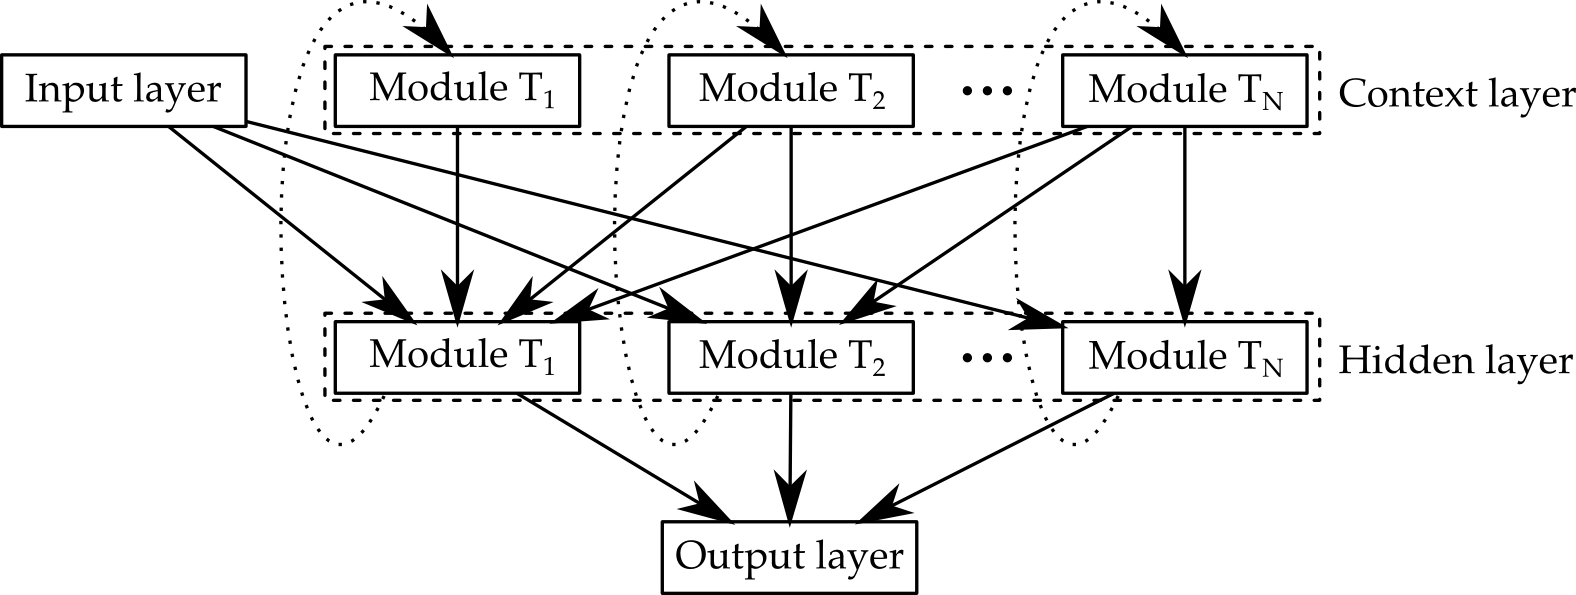
\includegraphics[width=394px]{cw-rnn.png}
		\caption{Clockwork-RNN. }
	\end{figure}
This allows slower modules to focus on long-term information in the input sequence, while faster modules focus on short-term information with context provided by slower modules. \par

To adapt network weights, BPTT learning algorithm can be used. The algorithm works similarly with the only difference compared to SRN being that error propagates only from active modules executed at time $t$. Error of inactive modules is retained from previous step. \par
%fewer parameters/weights
      
\chapter{Implementation}
\section{Neural Prediction Framework}
Neural Prediction Framework (NPF) is a tool built for experimenting with various neural network models in online time series prediction tasks.

\subsection{MemoryBlock}
MemoryBlock is an object encapsulating an array of floating point numbers and providing convenience methods. MemoryBlock is used all around NPF to store data points, network weights or activations. MemoryBlockView inherits from MemoryBlock and provides access to its elements inside specified range.
\subsection{NeuralLayer}
NeuralLayer is an object storing activation of units in a single layer and weights of connections coming from units of other layers. NeuralLayer is also capable of propagating input signals forward and propagating errors backward using standard backpropagation algorithm.
\subsection{NeuralNetwork}
NeuralNetwork is an abstract class providing common interface shared between all derived networks.
\subsection{FeedforwardNetwork}
FeedForwardNetwork implements a MLP with variable number of hidden layers with variable number of units in them.
\subsection{CWRecurrentNetwork}
CWRecurrentNetwork implements a CW-RNN with variable number of hidden layer modules with specified clock rates.
\subsection{SimpleRecurrentNetwork}
SimpleRecurrentNetwork derives from CWRecurrentNetwork to implement a SRN, since Elman's SRN is just a special case of CW-RNN network with single hidden layer module with clock rate equal one.
\subsection{LearningAlgorithm}
LearningAlgorithm is an abstract class providing common interface for all learning algorithms.
\subsection{Backpropagation, TBPTT, RTRL}
Backpropagation, TBPTT, RTRL classes are descendants of LearningAlgorithm implementing respectively named algorithms. Backpropagation class is used for training a FeedforwardNetwork. RTRL is capable of training a SimpleRecurrentNetwork. TBPTT supports both SimpleRecurrentNetwork and CWRecurrentNetwork.

\section{Network Monitor}
Network monitor works with assistance of unix system resources monitoring tool Dstat \cite{dstat}. Output of Dstat is redirected to a neural network of choice for prediction. As a proof of concept, the network is constantly training and predicting incoming and outgoing network traffic. Should the difference between prediction and actual value exceed predefined threshold, this incident is logged to a file as an anomaly.
\section{Robotic Arm Simulator}
Robotic arm simulator is implemented in BEPUPhysics 3D physics library \cite{bepuphysics}. Manipulator with three degrees of freedom from BEPU demo is constructed in 3D world. Three controlled joints are situated in base, "shoulder" and "elbow" of the arm. Simulator renders the scene, calculates physics and supplies information about current rotation of joints as well as position of claw to NPF, which provides prediction of claw position in next time step. As a proof of concept, line showing direction from current position of claw to the predicted position is drawn. Further use could be found in control of the arm.
	\begin{figure}[ht]
		\centering
		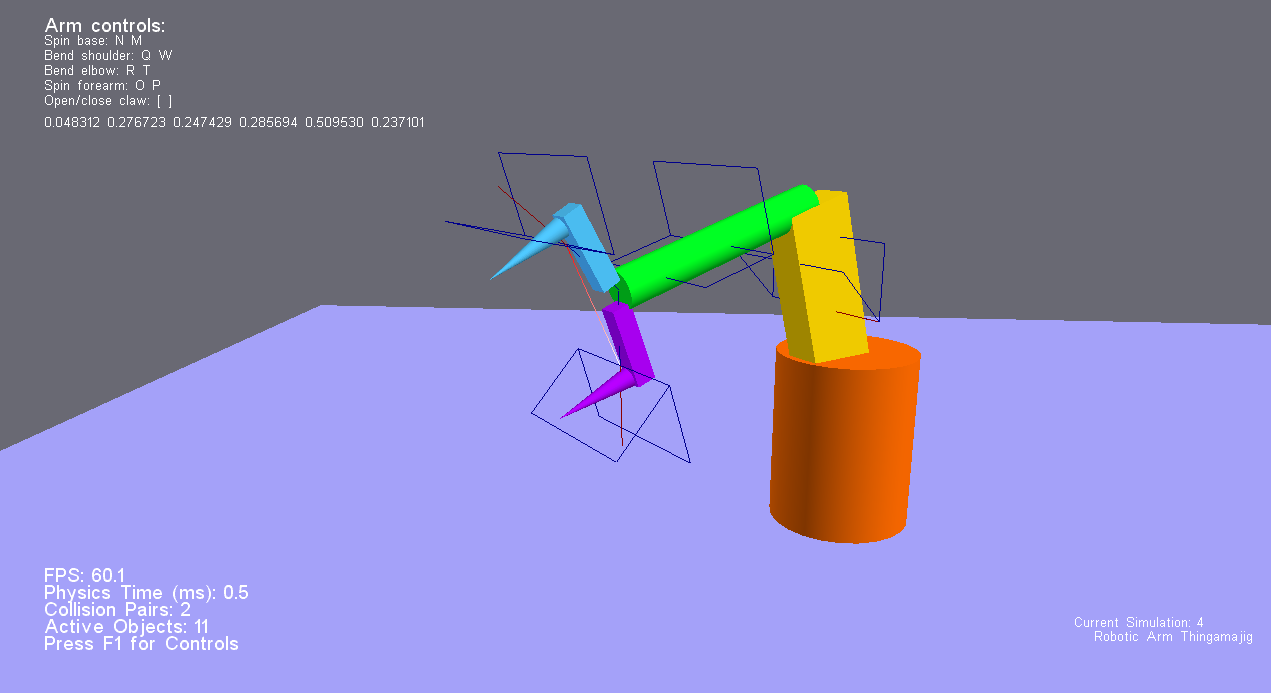
\includegraphics[width=360px]{roboticarm.png}
		\caption{Robotic arm in BEPUPhysics 3D physics simulator.}
	\end{figure}

\chapter{Experiments}
In the following experiments, I attempt to find the best performing network and its hyperparameters for prediction in three different scenarios with restricted computation time.\par

Networks are tested on the same prepared datasets to ensure equal testing conditions. Units of all networks use logistic activation function. Weights of connections in all networks are initialised randomly with uniform distribution on interval [-0.25, 0.25]. Since the initial setting of network influences its overall performance, all experiments described below are run ten times and only the average of them is presented as the result.\par

Experiments measuring computation time are run on 1.7GHz Intel Core i5 2557M. While the absolute computation times should vary depending on system configuration, I expect them to retain their ratio relative to each other.\par

As a measure of prediction accuracy, total error $E_{total}$ collected over $T$ time steps is used. Network that predicts entire sequence flawlessly would have zero total error. %mention higher worse?
$$E_{total} = \sum\limits_{\tau = 1}^T {1 \over 2} \sum\limits_{i=1}^{n}\left(Target_i - Output_i\right)^2$$
Networks are trained online in every time step. In order to capture both their accuracy and ability to adapt quickly, there is no traditional division into training and testing period. Instead, networks are evaluated online as they learn in all time steps.

\section{Testing Scenarios}
Networks are tested on three different datasets with varying complexity collected from three scenarios. Each scenario is designed to test a specific aspect of prediction, such as modelling generative processes, noisy network traffic or substantially time constrained robotic manipulator.
\subsection{Goniometric function}
The first simple testing scenario is predicting next step of a generative process with no inputs whose output in time $t$ is defined as
$$Output_t ={{1 + sin(t)cos(2t)} \over 2}$$

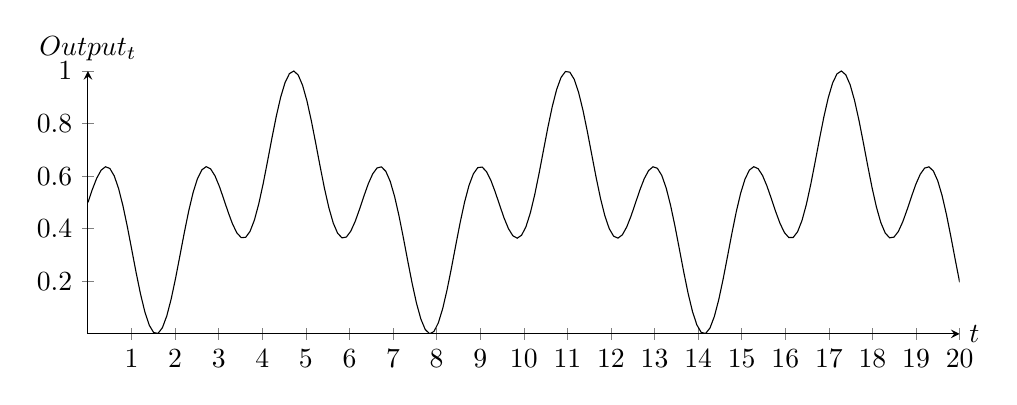
\begin{tikzpicture}[domain=0:20,samples=200]
\begin{axis}[
  axis x line=middle,
  axis y line=middle,
  xmin=0, xmax=20,
  ymin=0, ymax=1,
  height=140,
  width=360,
  xtick={0,1,...,20},
  ytick={0,0.2,...,1},
  xlabel={$t$},
  ylabel={$Output_t$},
  xlabel style={right},
  ylabel style={above},
]
\addplot[]{0.5 + 0.5*sin(deg(x))*cos(deg(2*x))};
\end{axis}
\end{tikzpicture}

The goniometric function's range is [0,1] which matches logistic activation function's range [0,1], therefore no preprocessing is needed. This function is periodical with period of $2\pi$.

\subsection{Network Usage}
Second testing scenario is predicting computer network usage measured by monitoring tool Dstat. Each second, Dstat measures usage of system resources such as CPU load, memory usage, disk throughput, number of open sockets as well as network incoming and outgoing traffic. Prediction has to be computed in less time than it takes Dstat to collect network usage, which poses a loose time constraint of computation time being less than one second. Dataset consists of 3,600 data points created by monitoring real application server for one hour.\par
Dstat measures 26 variables of the monitored system, two of which are incoming and outgoing network traffic. Values of these two variables in next time step shall be predicted. Since the values observed by Dstat have huge dynamic range, preprocessing is necessary. Values are linearly squashed into interval [0, 1] by dividing the observed value by the expected maximum.
\subsection{Robotic Arm}
Third testing scenario is predicting position of robotic arm's claw in BEPUPhysics 3D physics library. Manipulator with three controlled joints is constructed. At each simulation step, network receives rotations of all joints and their respective control signals. The goal is to predict next position of the claw in 3D coordinate system.\par
This task is heavily time constrained. The 3D simulator is required to run at 60 frames per second for smooth control, which leaves only $1 \over 60$ of a second for computation of the prediction. Dataset consisting of 18,000 data points is created by controlling the robot with random commands for a period of five minutes.

\section{Time-Delay Neural Network Experiments}
Following experiments examine role of sliding window size and number of hidden units on network's performance. Network with one hidden layer with 128, 256 and 512 hidden units is tested with sliding windows of various sizes to determine their impact on performance and computation time. Learning and momentum rates are informally chosen to the best performing value for each dataset.

\subsection{Precision of Predicting Goniometric Function}
Networks are tested with learning and momentum rate equal 0.05 and 0.9 respectively. The results show steep decrease of error when increasing window size from two to three past time steps and mild decrease of error when increasing window size further. Presumably, three steps are enough to capture dynamics of a simple goniometric function. Number of hidden units has little effect.

\begin{figure}[H]
\centering
\caption{Total error of predicting goniometric function with TDNN and various sliding window sizes.}
\begin{tikzpicture}
	\begin{axis}[
	  xlabel=Sliding window size,
	  ylabel=Total error,
	  xmin = 0,
	  ymin = 0,
	  axis lines = left,
	  xtick={1,2,...,20},
 	  ytick={0,10,...,60},
	  legend pos=north east,
	  height=180,
	  width=360]
 	\addplot table [x=WS, y=ERROR64]{tdnn_gon_error.dat};
	\addlegendentry{64 hidden units}
	\addplot table [x=WS, y=ERROR128]{tdnn_gon_error.dat};
	\addlegendentry{128 hidden units}
	\addplot table [x=WS, y=ERROR256]{tdnn_gon_error.dat};
	\addlegendentry{256 hidden units}
	\end{axis}
\end{tikzpicture}
\end{figure}

\subsection{Precision of Predicting Network Usage}
Networks with 128, 256 and 512 units in single hidden layer are tested with learning and momentum rate equal 0.001 and 0.9 respectively. Sliding window size and number of hidden units show little or no effect on reducing total error. This behaviour could be caused by inherent unpredictability of the network traffic.


\begin{figure}[H]
\centering
\caption{Total error of predicting network traffic with TDNN and various sliding window sizes.}
\begin{tikzpicture}
	\begin{axis}[
	  xlabel=Sliding window size,
	  ylabel=Total error,
	  xmin = 0,
	  ymin = 0,
	  ymax=65,
	  axis lines = left,
%	  xtick={1,2,...,20},
%	  ytick={0,10,...,70},
	  legend pos=south east,
	  height=180,
	  width=360]
	 \addplot table [x=WS, y=ERROR64]{tdnn_net_error.dat};
	\addlegendentry{64 hidden units}
	\addplot table [x=WS, y=ERROR128]{tdnn_net_error.dat};
	\addlegendentry{128 hidden units}
	\addplot table [x=WS, y=ERROR256]{tdnn_net_error.dat};
	\addlegendentry{256 hidden units}
	\end{axis}
\end{tikzpicture}
\end{figure}

\subsection{Precision of Predicting Position of Manipulator's Claw}
Networks with 128, 256 and 512 units in single hidden layer are tested with learning and momentum rate equal 0.01 and 0.9 respectively. Regardless of number of units, networks find their error minimum with window of size two or three. Enlarging the  window further has negative impact and increases error. The larger the network, the more susceptible it is to this. This may suggest that the state of manipulator is sufficiently captured in two or three consecutive steps.

\begin{figure}[H]
\centering
\caption{Total error of predicting manipulator's claw position with TDNN and various sliding window sizes.}
\begin{tikzpicture}
	\begin{axis}[
	  xlabel=Sliding window size,
	  ylabel=Total error,
	  xmin = 0,
	  ymin = 0,
	  %ymax=65,
	  axis lines = left,
%	  xtick={1,2,...,20},
	  ytick={0,10,...,120},
	  legend pos=south east,
	  height=180,
	  width=360]
  	\addplot table [x=WS, y=ERROR64]{tdnn_man_error.dat};
	\addlegendentry{64 hidden units}
	\addplot table [x=WS, y=ERROR128]{tdnn_man_error.dat};
	\addlegendentry{128 hidden units}
	\addplot table [x=WS, y=ERROR256]{tdnn_man_error.dat};
	\addlegendentry{256 hidden units}
	\end{axis}
\end{tikzpicture}
\end{figure}

\subsection{Computation Time}
As expected, increasing window size is linearly increasing the computation time. Similarly, computation time is increased linearly by adding hidden units.

\begin{figure}[H]
\centering
\caption{Computation time of predicting goniometric function with TDNN and various sliding window sizes.}
\begin{tikzpicture}
	\begin{axis}[
	  xlabel=Sliding window size,
	  ylabel=Time (s),
	  xmin = 0,
	  ymin = 0,
	  axis lines = left,
	  xtick={0,2,...,20},
	  legend pos=north west,
	  height=180,
	  width=360]
  	\addplot table [x=WS, y=TIME64]{tdnn_gon_time.dat};
	\addlegendentry{64 hidden units}
	\addplot table [x=WS, y=TIME128]{tdnn_gon_time.dat};
	\addlegendentry{128 hidden units}
	\addplot table [x=WS, y=TIME256]{tdnn_gon_time.dat};
	\addlegendentry{256 hidden units}
	\end{axis}
\end{tikzpicture}
\end{figure}

\begin{figure}[H]
\centering
\caption{Computation time of predicting network traffic with TDNN and various sliding window sizes.}
\begin{tikzpicture}
	\begin{axis}[
	  xlabel=Sliding window size,
	  ylabel=Time (s),
	  xmin = 0,
	  ymin = 0,
	  axis lines = left,
%	  xtick={0,2,...,20},
%	  ytick={0,0.1,...,0.2},
	  legend pos=north west,
	  height=180,
	  width=360]
  	\addplot table [x=WS, y=TIME64]{tdnn_net_time.dat};
	\addlegendentry{64 hidden units}
	\addplot table [x=WS, y=TIME128]{tdnn_net_time.dat};
	\addlegendentry{128 hidden units}
	\addplot table [x=WS, y=TIME256]{tdnn_net_time.dat};
	\addlegendentry{256 hidden units}
	\end{axis}
\end{tikzpicture}
\end{figure}


\begin{figure}[H]
\centering
\caption{Computation time of predicting manipulator's claw position with TDNN and various sliding window sizes.}
\begin{tikzpicture}
	\begin{axis}[
	  xlabel=Sliding window size,
	  ylabel=Time (s),
	  xmin = 0,
	  ymin = 0,
	  axis lines = left,
%	  xtick={0,2,...,20},
%	  ytick={0,0.1,...,0.2},
	  legend pos=north west,
	  height=180,
	  width=360]
  	\addplot table [x=WS, y=TIME64]{tdnn_man_time.dat};
	\addlegendentry{64 hidden units}
	\addplot table [x=WS, y=TIME128]{tdnn_man_time.dat};
	\addlegendentry{128 hidden units}
	\addplot table [x=WS, y=TIME256]{tdnn_man_time.dat};
	\addlegendentry{256 hidden units}
	\end{axis}
\end{tikzpicture}
\end{figure}

\section{Truncated Backpropagation Through Time Experiments}
Following experiments examine role of unfolding depth and number of hidden units on network's precision and computation time. Learning and momentum rates are informally chosen to the best performing value for each dataset.

\subsection{Precision of Predicting Goniometric Function}
As unfolding depth increases, total errors of the networks are oscillating with period of roughly $2\pi$, the reason of which is unclear to me.

\begin{figure}[H]
\centering
\caption{Total error of predicting goniometric function with SRN trained by TBPTT with various unfolding depth.}
\begin{tikzpicture}
	\begin{axis}[
	  xlabel=Unfolding depth,
	  ylabel=Total error,
	  xmin = 0,
	  ymin = 0,
	  axis lines = left,
	  xtick={1,2,...,20},
 	  ytick={0,10,...,60},
	  legend pos=south west,
	  height=180,
	  width=360]
	\addplot table [x=WS, y=ERROR64]{tbptt_gon_error.dat};
	\addlegendentry{64 hidden units}
	\addplot table [x=WS, y=ERROR128]{tbptt_gon_error.dat};
	\addlegendentry{128 hidden units}
	\addplot table [x=WS, y=ERROR256]{tbptt_gon_error.dat};
	\addlegendentry{256 hidden units}
	\end{axis}
\end{tikzpicture}
\end{figure}

\subsection{Precision of Predicting Network Traffic}
Total errors of the networks find their minimum with unfolding depth between two and six and then the trend is upward. Similar to TDNN, the effect of adding more hidden units is questionable.

\begin{figure}[H]
\centering
\caption{Total error of predicting network traffic with SRN trained by TBPTT with various unfolding depth.}
\begin{tikzpicture}
	\begin{axis}[
	  xlabel=Unfolding depth,
	  ylabel=Total error,
	  xmin = 0,
	  ymin = 0,
	  axis lines = left,
	  xtick={1,2,...,20},
 	  ytick={0,10,...,60},
	  legend pos=south west,
	  height=180,
	  width=360]
	\addplot table [x=WS, y=ERROR64]{tbptt_net_error.dat};
	\addlegendentry{64 hidden units}
	\addplot table [x=WS, y=ERROR128]{tbptt_net_error.dat};
	\addlegendentry{128 hidden units}
	\addplot table [x=WS, y=ERROR256]{tbptt_net_error.dat};
	\addlegendentry{256 hidden units}
	\end{axis}
\end{tikzpicture}
\end{figure}

\subsection{Precision of Predicting Position of Manipulator's Claw}
The number of hidden units is clearly decreasing total error with any unfolding depth. Total errors find their minimum to be roughly in the middle of the tested interval.

\begin{figure}[H]
\centering
\caption{Total error of predicting manipulator's claw position with SRN trained by TBPTT with various unfolding depth.}
\begin{tikzpicture}
	\begin{axis}[
	  xlabel=Unfolding depth,
	  ylabel=Total error,
	  xmin = 0,
	  ymin = 0,
	  axis lines = left,
	  xtick={1,2,...,20},
 	  ytick={0,25,...,220},
	  legend pos=north east,
	  height=180,
	  width=360]
	\addplot table [x=WS, y=ERROR64]{tbptt_man_error.dat};
	\addlegendentry{64 hidden units}
	\addplot table [x=WS, y=ERROR128]{tbptt_man_error.dat};
	\addlegendentry{128 hidden units}
	\addplot table [x=WS, y=ERROR256]{tbptt_man_error.dat};
	\addlegendentry{256 hidden units}
	\end{axis}
\end{tikzpicture}
\end{figure}

\subsection{Computation Time}
Increasing unfolding linearly increases the computation time. On the other had, computation time is increased quadratically by adding more hidden units.

\begin{figure}[H]
\centering
\caption{Computation time of predicting goniometric function with SRN trained by TBPTT with various unfolding depth.}
\begin{tikzpicture}
	\begin{axis}[
	  xlabel=Unfolding depth,
	  ylabel=Time (s),
	  xmin = 0,
	  ymin = 0,
	  axis lines = left,
	  xtick={0,2,...,20},
	  legend pos=north west,
	  height=180,
	  width=360]
	\addplot table [x=WS, y=TIME64]{tbptt_gon_time.dat};
	\addlegendentry{64 hidden units}
	\addplot table [x=WS, y=TIME128]{tbptt_gon_time.dat};
	\addlegendentry{128 hidden units}
	\addplot table [x=WS, y=TIME256]{tbptt_gon_time.dat};
	\addlegendentry{256 hidden units}
	\end{axis}
\end{tikzpicture}
\end{figure}

\begin{figure}[H]
\centering
\caption{Computation time of predicting network traffic with SRN trained by TBPTT with various unfolding depth.}
\begin{tikzpicture}
	\begin{axis}[
	  xlabel=Unfolding depth,
	  ylabel=Time (s),
	  xmin = 0,
	  ymin = 0,
	  axis lines = left,
	  xtick={0,2,...,20},
	  legend pos=north west,
	  height=180,
	  width=360]
	\addplot table [x=WS, y=TIME64]{tbptt_net_time.dat};
	\addlegendentry{64 hidden units}
	\addplot table [x=WS, y=TIME128]{tbptt_net_time.dat};
	\addlegendentry{128 hidden units}
	\addplot table [x=WS, y=TIME256]{tbptt_net_time.dat};
	\addlegendentry{256 hidden units}
	\end{axis}
\end{tikzpicture}
\end{figure}

\begin{figure}[H]
\centering
\caption{Computation time of predicting manipulator's claw position with SRN trained by TBPTT with various unfolding depth.}
\begin{tikzpicture}
	\begin{axis}[
	  xlabel=Unfolding depth,
	  ylabel=Time (s),
	  xmin = 0,
	  ymin = 0,
	  axis lines = left,
	  xtick={0,2,...,20},
	  legend pos=north west,
	  height=180,
	  width=360]
	\addplot table [x=WS, y=TIME64]{tbptt_man_time.dat};
	\addlegendentry{64 hidden units}
	\addplot table [x=WS, y=TIME128]{tbptt_man_time.dat};
	\addlegendentry{128 hidden units}
	\addplot table [x=WS, y=TIME256]{tbptt_man_time.dat};
	\addlegendentry{256 hidden units}
	\end{axis}
\end{tikzpicture}
\end{figure}

\section{Real-Time Recurrent Learning Experiments}
The impact of hidden layer size of a SRN trained by RTRL on precision and computation time is examined. Networks with only 8 and 16 hidden units are tested due to high computation time exceeding limits of all scenarios. Learning rate is set to 0.1 and momentum rate to 0.9. 

\subsection{Precision of Prediction}
The error trend goes slightly downward with increasing number of units, but because there are so few of them, maximum achievable precision is limited.

\begin{figure}[H]
\centering
\caption{Total error of prediction in all three scenarios with SRN trained by RTRL with various number of hidden units.}
\begin{tikzpicture}
	\begin{axis}[
	  xlabel=Hidden units,
	  ylabel=Total error,
	  xmin = 0,
	  ymin = 0,
	  axis lines = left,
 	  xtick={8,16},
	  legend pos=north west,
	  height=180,
	  width=360]
	\addplot table [x=N, y=ERRORG]{rtrl_error.dat};
	\addlegendentry{Goniometric function}
	\addplot table [x=N, y=ERRORN]{rtrl_error.dat};
	\addlegendentry{Network usage}
	\addplot table [x=N, y=ERRORM]{rtrl_error.dat};
	\addlegendentry{Manipulator}
	\end{axis}
\end{tikzpicture}
\end{figure}

\subsection{Computation Time}
RTRL's $O(n^4)$ time complexity appears to be the limiting factor in online use. Even with 16 hidden units, the network approaches maximum allowed execution time of 360 seconds in manipulator scenario.

\begin{figure}[H]
\centering
\caption{Computation time of prediction in all three scenarios with SRN trained by RTRL with various number of hidden units.}
\begin{tikzpicture}
	\begin{axis}[
	  xlabel=Hidden units,
	  ylabel=Total error,
	  xmin = 0,
	  ymin = 0,
	  axis lines = left,
 	  xtick={8,16},
	  legend pos=north west,
	  height=180,
	  width=360]
	\addplot table [x=N, y=TIMEG]{rtrl_time.dat};
	\addlegendentry{Goniometric function}
	\addplot table [x=N, y=TIMEN]{rtrl_time.dat};
	\addlegendentry{Network usage}
	\addplot table [x=N, y=TIMEM]{rtrl_time.dat};
	\addlegendentry{Manipulator}
	\end{axis}
\end{tikzpicture}
\end{figure}




\section{Clockwork Recurrent Network Experiments}
Following experiments examine role of unfolding depth and number of hidden units in CW-RNN on its precision and computation time. Learning and momentum rates are informally chosen to the best performing value for each dataset. Hidden layer of tested network is divided into four equally big modules with periods 1, 2, 4 and 8.

\subsection{Precision of Predicting Goniometric Function}
As unfolding depth increases, total errors of the networks are oscillating with period of roughly $2\pi$, the reason of which is unclear to me.

\begin{figure}[H]
\centering
\caption{Total error of predicting goniometric function with CW-RNN trained by TBPTT with various unfolding depth.}
\begin{tikzpicture}
	\begin{axis}[
	  xlabel=Unfolding depth,
	  ylabel=Total error,
	  xmin = 0,
	  ymin = 0,
	  axis lines = left,
	  xtick={1,2,...,20},
 	  ytick={0,10,...,60},
	  legend pos=south west,
	  height=180,
	  width=360]
	\addplot table [x=WS, y=ERROR64]{cw_gon_error.dat};
	\addlegendentry{64 hidden units}
	\addplot table [x=WS, y=ERROR128]{cw_gon_error.dat};
	\addlegendentry{128 hidden units}
	\addplot table [x=WS, y=ERROR256]{cw_gon_error.dat};
	\addlegendentry{256 hidden units}
	\end{axis}
\end{tikzpicture}
\end{figure}

\subsection{Precision of Predicting Network Traffic}
Total errors of the networks find their minimum with small unfolding depth value and then the trend is upward. Similar to TDNN, the effect of adding more hidden units is questionable.

\begin{figure}[H]
\centering
\caption{Total error of predicting network traffic with CW-RNN trained by TBPTT with various unfolding depth.}
\begin{tikzpicture}
	\begin{axis}[
	  xlabel=Unfolding depth,
	  ylabel=Total error,
	  xmin = 0,
	  ymin = 0,
	  axis lines = left,
	  xtick={1,2,...,20},
 	  ytick={0,10,...,60},
	  legend pos=south west,
	  height=180,
	  width=360]
	\addplot table [x=WS, y=ERROR64]{cw_net_error.dat};
	\addlegendentry{64 hidden units}
	\addplot table [x=WS, y=ERROR128]{cw_net_error.dat};
	\addlegendentry{128 hidden units}
	\addplot table [x=WS, y=ERROR256]{cw_net_error.dat};
	\addlegendentry{256 hidden units}
	\end{axis}
\end{tikzpicture}
\end{figure}

\subsection{Precision of Predicting Position of Manipulator's Claw}
The number of hidden units is clearly decreasing total error with any unfolding depth. Total errors find their minimum to be roughly in the middle of the tested interval.

\begin{figure}[H]
\centering
\caption{Total error of predicting manipulator's claw position with CW-RNN trained by TBPTT with various unfolding depth.}
\begin{tikzpicture}
	\begin{axis}[
	  xlabel=Unfolding depth,
	  ylabel=Total error,
	  xmin = 0,
	  ymin = 0,
	  axis lines = left,
	  xtick={1,2,...,20},
	  ytick={0,25,...,225},
	  legend pos=north east,
	  height=180,
	  width=360]
	\addplot table [x=WS, y=ERROR64]{cw_man_error.dat};
	\addlegendentry{64 hidden units}
	\addplot table [x=WS, y=ERROR128]{cw_man_error.dat};
	\addlegendentry{128 hidden units}
	\addplot table [x=WS, y=ERROR256]{cw_man_error.dat};
	\addlegendentry{256 hidden units}
	\end{axis}
\end{tikzpicture}
\end{figure}

\subsection{Computation Time}
Increasing unfolding linearly increases the computation time. On the other had, computation time is increased quadratically by adding more hidden units. Interestingly, the computation time of CW-RNN is approximately half of that of SRN.

\begin{figure}[H]
\centering
\caption{Computation time of predicting goniometric function with CW-RNN trained by TBPTT with various unfolding depth.}
\begin{tikzpicture}
	\begin{axis}[
	  xlabel=Unfolding depth,
	  ylabel=Time (s),
	  xmin = 0,
	  ymin = 0,
	  axis lines = left,
	  xtick={0,2,...,20},
	  legend pos=north west,
	  height=180,
	  width=360]
	\addplot table [x=WS, y=TIME64]{cw_gon_time.dat};
	\addlegendentry{64 hidden units}
	\addplot table [x=WS, y=TIME128]{cw_gon_time.dat};
	\addlegendentry{128 hidden units}
	\addplot table [x=WS, y=TIME256]{cw_gon_time.dat};
	\addlegendentry{256 hidden units}
	\end{axis}
\end{tikzpicture}
\end{figure}

\begin{figure}[H]
\centering
\caption{Computation time of predicting network traffic with CW-RNN trained by TBPTT with various unfolding depth.}
\begin{tikzpicture}
	\begin{axis}[
	  xlabel=Unfolding depth,
	  ylabel=Time (s),
	  xmin = 0,
	  ymin = 0,
	  axis lines = left,
	  xtick={0,2,...,20},
	  legend pos=north west,
	  height=180,
	  width=360]
	\addplot table [x=WS, y=TIME64]{cw_net_time.dat};
	\addlegendentry{64 hidden units}
	\addplot table [x=WS, y=TIME128]{cw_net_time.dat};
	\addlegendentry{128 hidden units}
	\addplot table [x=WS, y=TIME256]{cw_net_time.dat};
	\addlegendentry{256 hidden units}
	\end{axis}
\end{tikzpicture}
\end{figure}

\begin{figure}[H]
\centering
\caption{Computation time of predicting manipulator's claw position with CW-RNN trained by TBPTT with various unfolding depth.}
\begin{tikzpicture}
	\begin{axis}[
	  xlabel=Unfolding depth,
	  ylabel=Time (s),
	  xmin = 0,
	  ymin = 0,
	  axis lines = left,
	  xtick={0,2,...,20},
	  ytick={0,25,...,125},
	  legend pos=north west,
	  height=180,
	  width=360]
	\addplot table [x=WS, y=TIME64]{cw_man_time.dat};
	\addlegendentry{64 hidden units}
	\addplot table [x=WS, y=TIME128]{cw_man_time.dat};
	\addlegendentry{128 hidden units}
	\addplot table [x=WS, y=TIME256]{cw_man_time.dat};
	\addlegendentry{256 hidden units}
	\end{axis}
\end{tikzpicture}
\end{figure}


\chapter{Results}
TODO
\section{Trade-offs}
TODO

\chapter{Conclusion}
TODO
%what is better at what


    \appendix
    \chapter{Appendix}
    Source code of all tested models and experiments can be found at https://github.com/karolkuna/Time-Series-Prediction-Using-Neural-Networks
    
    % Bibliography goes here
	\bibliographystyle{plain}
	\bibliography{bibliography}
    
    % Index goes here (optional)
\end{document}











